% !Mode:: "TeX:UTF-8"
\chapter{算法设计}
\section{车牌定位}
车牌定位就是采用一系列图像处理或者数学的方法从一幅图像中将车牌准确地定位出来。车牌定位提取出的车牌是整个车
牌识别系统的数据来源,它的效果的好坏直接影响到整个系统的表现,只有准确地定位出车牌,才会有后续的车牌分割与
字符识别。目前车牌定位有两大类、基于灰度、基于彩色。
\begin{figure}[h]
	\centering
	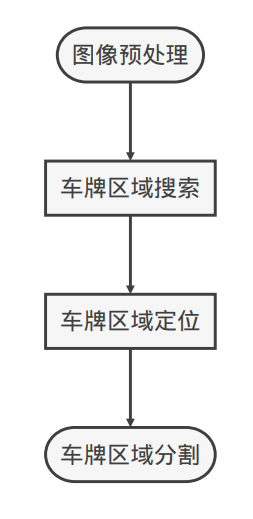
\includegraphics[scale=0.5]{figures/5.png}
	\caption{车牌定位流程图}
	\label{fig:2}
\end{figure}

详细步骤如图3.2
\begin{figure}[h]
	\centering
	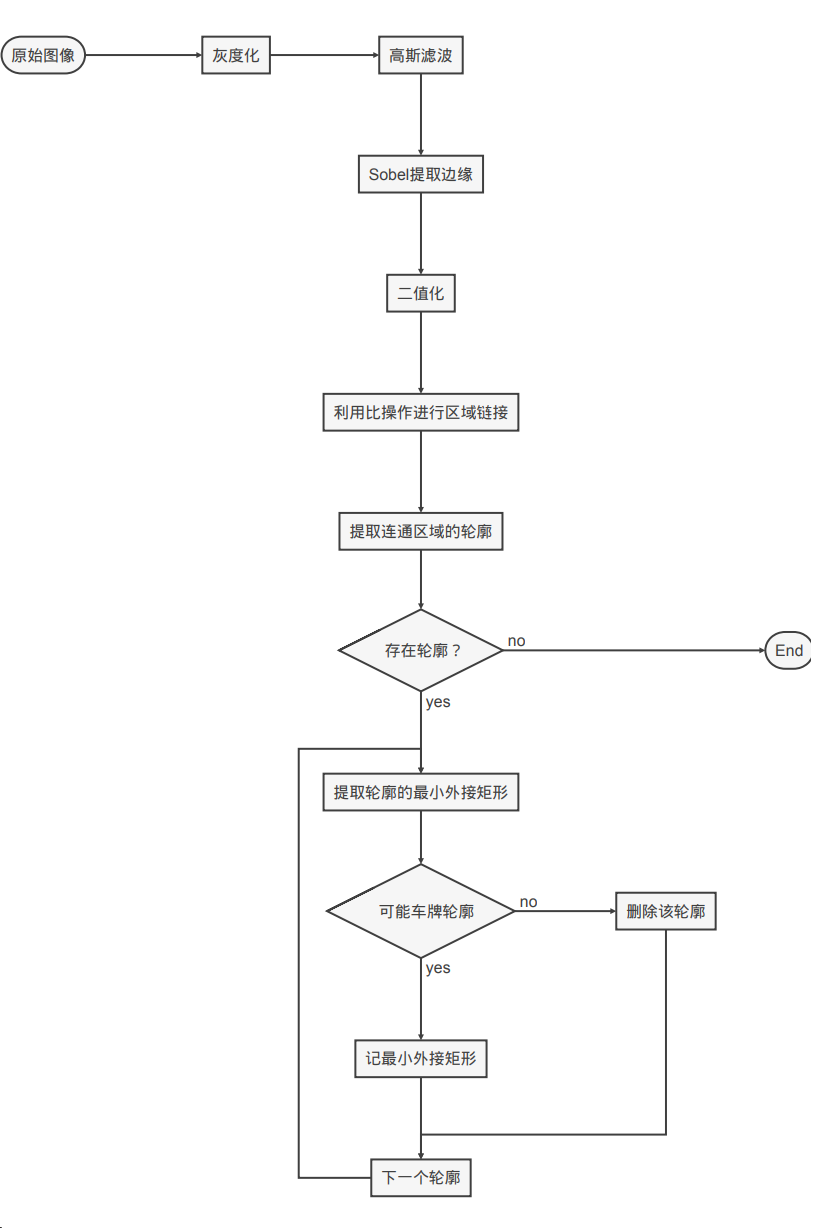
\includegraphics[scale=0.5]{figures/6.png}
	\caption{详细步骤}
	\label{fig:2}
\end{figure}


\section{字符分割}
字符分割算法流程同车牌分割不再详述,如图3.3
\begin{figure}[h]
	\centering
	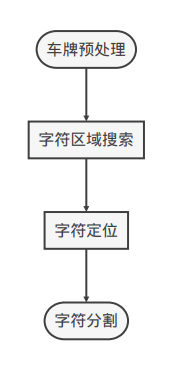
\includegraphics[scale=0.5]{figures/7.png}
	\caption{字符分割流程图}
	\label{fig:2}
\end{figure}

\section{重要步骤详述}
\subsection{旋转至水平方向}
如图3.4,$\theta>0$需要沿角度减小的方向旋转,$\theta<0$ 需要沿角度增大的方向旋转,因此旋转矩阵为:
\begin{equation}
\begin{aligned}
\left[
\begin{matrix}
x1\\
y1
\end{matrix}
\right]
=
\left[
\begin{matrix}
cos\theta & sin\theta\\
-sin\theta & cos\theta 
\end{matrix}
\right]
\left[
\begin{matrix}
x_0\\
y_0 
\end{matrix}
\right]
\Rightarrow
A(\theta)=
\left[
\begin{matrix}
cos\theta & sin\theta\\
-sin\theta & cos\theta 
\end{matrix}
\right] 
\end{aligned}
\end{equation}
\begin{figure}[h]
	\centering
	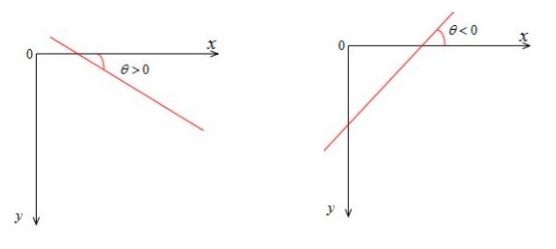
\includegraphics[scale=0.5]{figures/8.png}
	\caption{旋转水平方向}
	\label{fig:2}
\end{figure}


\subsection{旋转至垂直方向}
根据主轴方向求与y轴方向的夹角,其中$\beta$为与y正方向最小夹角,如果位于x轴正方向$\beta>0$,如果位于x轴反方向$\beta<0$。
\par
如图3.5,$\beta>0$需要沿角度增大的方向旋转,$\beta<0$ 需要沿角度减小的方向旋转,因此旋转矩阵为:
\begin{equation}
\begin{aligned}
\left[
\begin{matrix}
x1\\
y1
\end{matrix}
\right]
=
\left[
\begin{matrix}
cos\theta & -sin\theta\\
sin\theta & cos\theta 
\end{matrix}
\right]
\left[
\begin{matrix}
x_0\\
y_0 
\end{matrix}
\right]
\Rightarrow
B(\theta)=
\left[
\begin{matrix}
cos\theta & -sin\theta\\
sin\theta & cos\theta 
\end{matrix}
\right] 
\end{aligned}
\end{equation}
\begin{figure}[h]
	\centering
	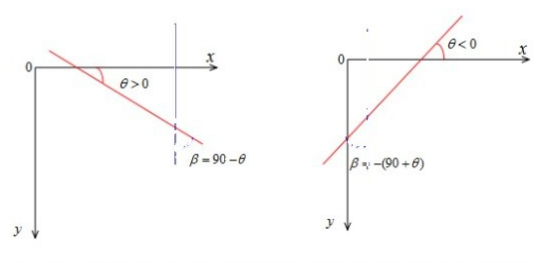
\includegraphics[scale=0.5]{figures/9.png}
	\caption{旋转垂直方向}
	\label{fig:2}
\end{figure}

由于$B(\theta)=A(\theta)$,也可以采用$A(\theta)$,只需要$\beta=-\beta$即可:
\begin{equation}
\left\{
\begin{array}{lr}
\beta=-(90-\theta) \quad \theta>0\\
\beta=90+\theta \quad \theta<0
\end{array}
\right.
\end{equation}

\subsection{求矩形长宽比}
\begin{enumerate}
	\item 求主轴方向$\theta$
	\item 根据旋转至水平或垂直方向,选择合适的旋转矩阵
	\begin{equation*}
	A
	=
	\left[
	\begin{matrix}
	a_{11} & a_{12}\\
	a_{21} & a_{22}
	\end{matrix}
	\right]	
	\end{equation*}
	\item 求取连通域边界全部坐标
	\item 求取最小外接矩形长宽比
\end{enumerate}
